\chapter{Grundlagen}
\label{chap:Grundlagen}

	\section{ Convolutional Autoencoder}
	\label{sec:StackedConvolutionalAutoencoder}
		\subsection{Autoencoder }			
			\begin{figure}[h]
				\centering
				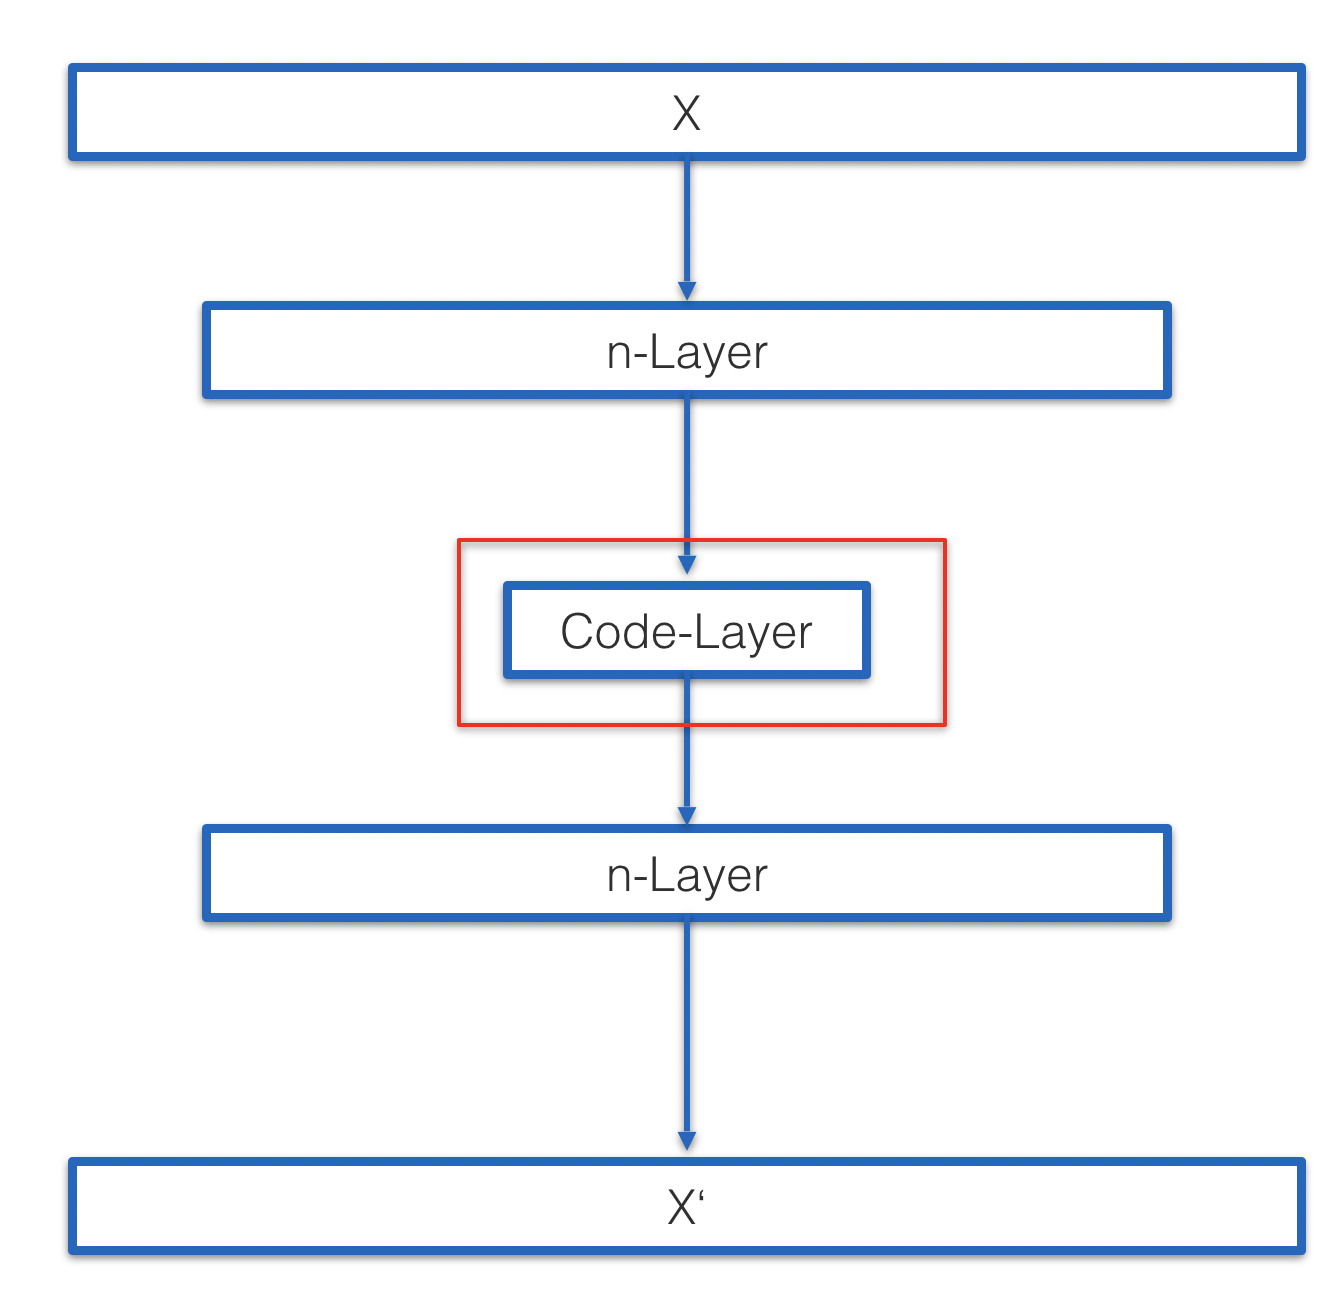
\includegraphics[width=0.5\textwidth, center]{bilder/Schema_Autoencoders/Schema_CAE.png}
				\caption[Schema Autoencoder]{Schema Autoencoder}
				\label{img:SchemaCAE}
			\end{figure}  
		
			- NN
		\subsection{Stacked Convolutional Autoencoder }
			, Convolutions nur per Quelle erläutern
		\subsection{Layerwise Pretrain }

		Warum pretrian?:	https://papers.nips.cc/paper/3048-greedy-layer-wise-training-of-deep-networks.pdf (Warum machen das andere heute nicht mehr? viele cnn haben vanishing gradients problem  über relu,... gelösst) (weitere literatur: möglicherweise Geoffrey E. Hinton)

		Stacked Convolutional Auto-Encoders Stacked Convolutional Auto-Encoders for
		Hierarchical Feature Extraction
		Jonathan Masci, Ueli Meier, Dan Ciresan, and Jurgen Schmidhuber
		Istituto Dalle Molle di Studi sullIntelligenza Artificiale (IDSIA)
		Lugano, Switzerland
		{jonathan,ueli,dan,juergen}@idsia.ch
		
		- layerwise pretrain {Greedy Layer-Wise Training of Deep Networks}
	\section{Transfer Learning}
	\label{sec:TransferLearning}
			oberste Schichten allgemeiner todo papaer verweisen
	\section{AutoML}
	\label{sec:AutoML}
		
		\subsection{RandomSearch }
		
		\subsection{HyperBand }

		\subsection{BOHB }


	\section{Bibliotheken und Werkzeuge}
	\label{sec:BibliothekenundWerkzeuge}
	Für den Praktischen Teil der Abschlussarbeit wurde insbesondere Cnvrg \cite{cnvrg.io.} genutzt. Cnvrg.io ist eine "full-stack Data Science Platform" welche Werkzeuge für die Erstellung, Verwaltung, Bereitstellung und Automatisierung von maschinellem Lernen bereitstellt. Cnvrg erlaubt es Arbeitsbereiche mittels Containern zu erstellen. Die Container können dabei auf Maschinen in Azure \cite{Micorsoft.2020} zugreifen. Für die Experimente wurde ein vorgefertiger Container mit einer tesla-k80 \cite{Nvidia.2020}, fünf CPUs und 49 GB Arbeitspeicher genutzt. 

	Für die Entwicklung wurden Python \cite{PythonSoftwareFoundation.2020}, Jupyter Notebooks \cite{ProjectJupyter} und das Framework Tensorflow \cite{MartinAbadi.2015}  genutzt. Die wichtigsten Bibliotheken für die Arbeit sind Keras \cite{Chollet.2015} , Numpy \cite{Oliphant.2006} , Matplotlib \cite{Hunter.2007} , scikit-learn \cite{Pedregosa.2011} , ConfigSpace \cite{Lindauer.8162019} , Bayesian Optimization and Hyperband \cite{StefanFalkner.2018} . 
	
	Für die Visualisierung von Bildeinbettung wurde das Werkzeug "PSIORI Visualizer" erweitert und eingesetzt. Der Visualizer erlaubt es Daten in 3D darzustellen, von verschiedenen Blickwinkel und Zoomstufen zu betrachten, zu Filtern und mit zusätzlichen Informationen zu versehen. 
	\begin{figure}[h]
		\centering
		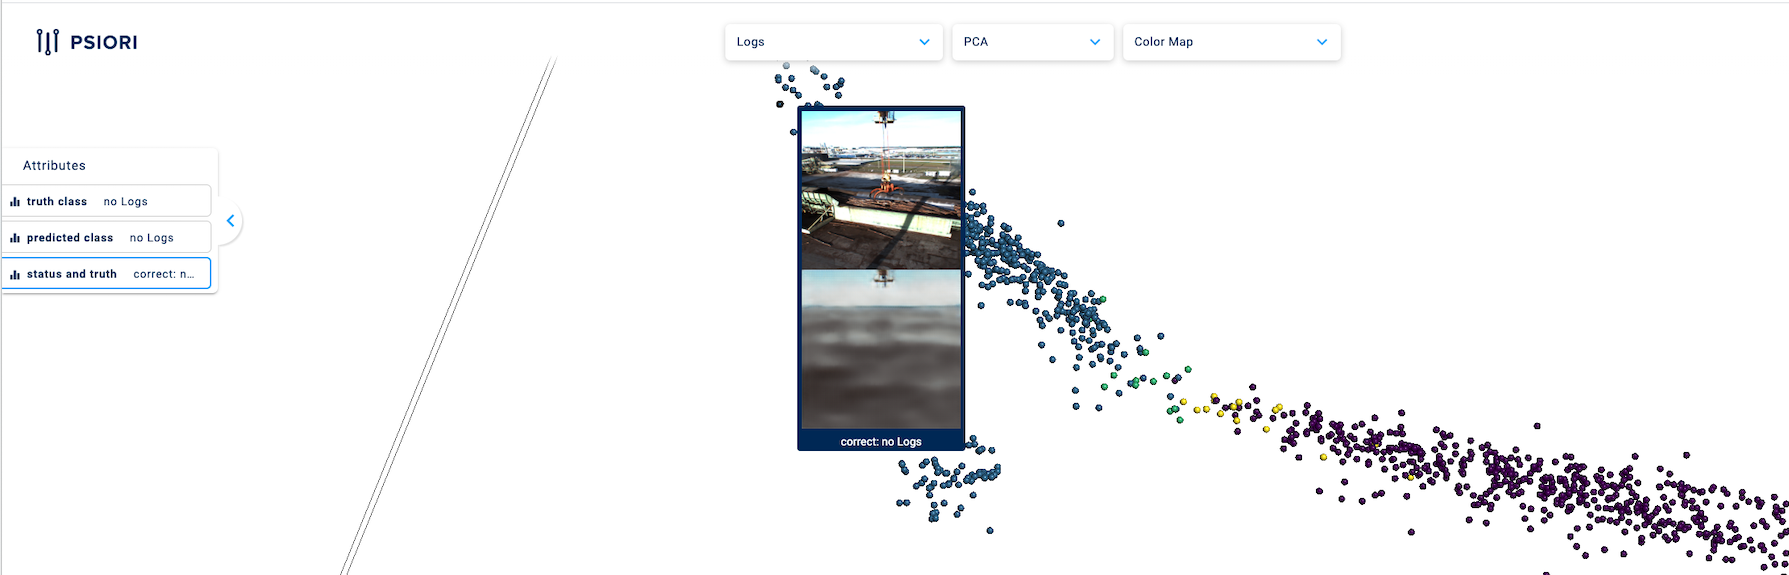
\includegraphics[width=1\textwidth, center]{bilder/Grundlagen/Example_Visualizer.png}
		\caption[Beispiel PSIORI Visualizer]{Beispiel PSIORI Visualizer}
		\label{img:ExampleVisualizer}
	\end{figure}  
	Die Abbildung \ref{img:ExampleVisualizer} zeigt einen Screenshot einer Visualisierung einer  Einbettung. Als zusätzliche Information sind die Datenpunkte entsprechend einer Klassifikation in True-Positiv, True-Negativ, False-Negativ und False-Positiv eingefärbt. Wird über einen Datenpunkt mit der Maus geschwebt, werden zusätliche Informationen zu dem Datenpunkt angezeigt. Diese Funktion wurde insbesondere zum Anzeigen eines Orginalbildes, ihrer Rekonstruktion mittels Autoencoder und einer Beschriftung  genutzt. 
	
	Kern der erstellten Werkzeuge ist das Framework  Psipy \cite{PSIORIGmbH.2019}. Psipy ist ein Python-Framework für Maschinelles Lernen welches von PSIORI selbst entwickelte Modelle zusammenfasst und eine einheitliche API zu Verfügung stellt. Diese API ist an die API des verbreiteten Frameworks scikit-learn angelehnt. Es können Modelle basierend auf scikit-learn  und Tensorflow eingebunden werden. 	
	In den nachfolgenden Abschnitten werden die, für die Arbeit, wichtigsten bestehenden Module des Frameworks vorgestellt.
	
	 \paragraph{saveable.py} Das Modul Saveable ist eine flexible Basisklasse die Kernfunktionalität zum Speichern und Laden von Python-Objekten bietet. Es können Modelle welche diverse Bibliotheken nutzen auf eine einheitliche Art und Weise gespeichert werden. Um die Klasse Saveable nutzen zu können, müssen erbende Klassen ihre Konstruktorargumente an die Basisklasse übergeben. Zusätlich ist es notwendig eine erweiterung beim Speichern und Laden zu implemmentieren. Beim Speichern ist es notwendig eine Erweiterung um alle (meist ein) Module und weitere Argumente zu implemmentieren. Beim Laden müssen die gespeicherten Module und Argumente geladen werden. In Listing \ref{lst:SaveTensorflow} ist die Erweiterung zum Speichern eines Tensorflow Models abgebildet. 
	\begin{lstlisting}[language=python,caption=Erweiterung zum Speichern eines Tensorflow Models, label=lst:SaveTensorflow]
		...
		zip_file.add("model.h5", self.model)
		...
	\end{lstlisting}

	\paragraph{autoencoder.py} Das Modul Autoencoder enthält die drei Klassen StackedAutoencoder, FullyConnectedAutoencoder und ConvolutionalAutoencoder. Der StackedAutoencoder wird als Basisklasse für die anderen beiden Klassen genutzt. Im Konstruktor werden Methoden aufgerufen welche in den abgeleiteten Klassen ausprogrammiert sind. Dabei wird ein Keras-Modell für einen Encoder und Decoder enstprechend von Parametern  erstellt. Als weitere wichtigen Methoden gibt es die Methode $pretrain(..)$ und $fit(..)$. Mittels $pretrain(..)$ werden die Schichten eines symmetrischer Autoencoder von aussen nach innen wie in 	\todo{Quelle Autoencoder pretrain} Greedy Layer-Wise Training of Deep Networks  vortrainiert. Die Auswahl der Schichten erfolgt wieder in den abgeleiteten Klassen.
	In der $fit(..)$-Methode wird nach einigen Prüfungen die Methode f$fit(..)$ 	\todo{Quelle fit Keras}	[fit Keras] des Kerasmodells aufgerufen. In Abbildung \ref{img:KlassendiagrammConvolutionalAutoencoder} ist das Klassendiagramm mit den öffnetlichen Methoden des ConvolutionalAutoencoder dargestellt. 
	\begin{figure}[h]
		\centering
		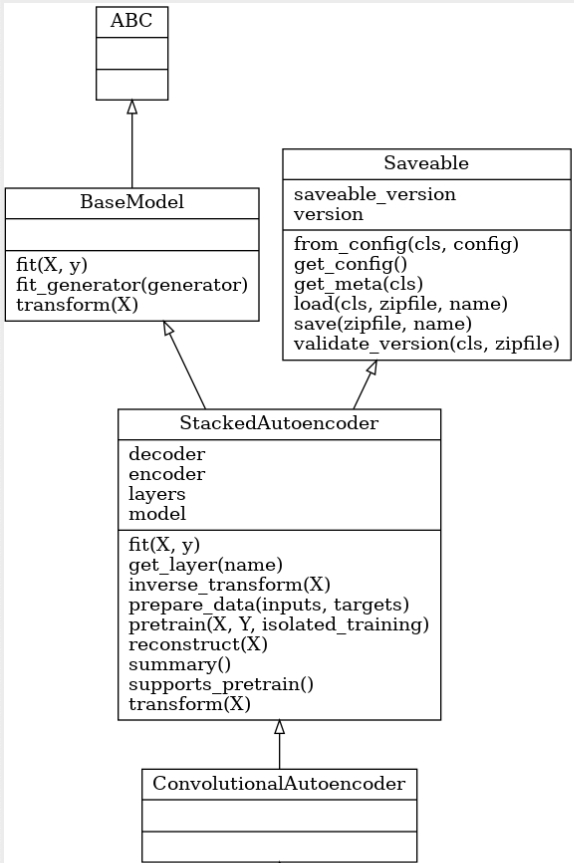
\includegraphics[width=0.5\textwidth, center]{bilder/Klassendiagramme/klassendiagramm_public_cae.png}
		\caption[Klassendiagramm ConvolutionalAutoencoder]{Klassendiagramm ConvolutionalAutoencoder}
		\label{img:KlassendiagrammConvolutionalAutoencoder}
	\end{figure}  
	
	\paragraph{hyperparameter\_mixin.py}  Hyperparameter\_mixin wird zum Standardisierten Verwalten von Hyperparametern für AutoML-Klassen genutzt. Auf die Hyperaparameter kann anschließend einheitlich zugegriffen werden. Abbildung \ref{img:KlassendiagrammHyperparametermixin}  zeigt das zugehörige UML-Klassendiagramm mit den Methoden zum Hinzufügen, Löschen und Laden der Hyperparameter. Da die Methoden öffentlich sind können über jede erbende Klasse die Hyperparameter eingenständig verwaltet werden.
	
	\begin{figure}[h]
		\centering
		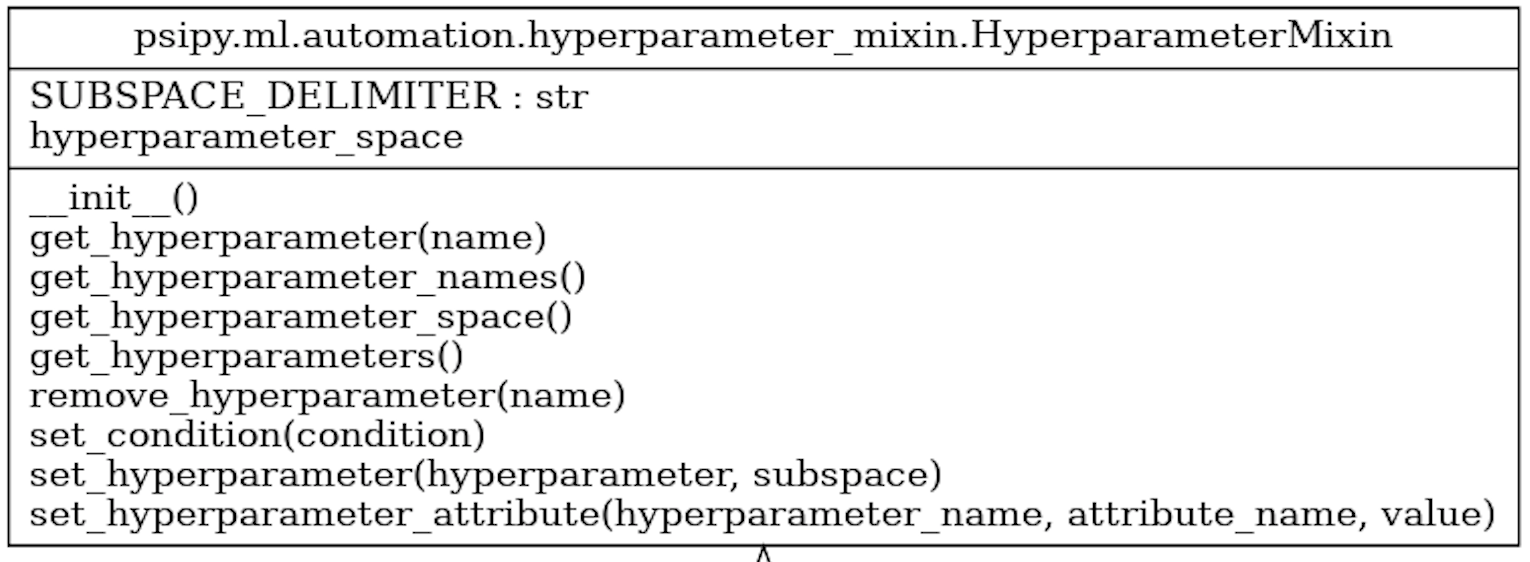
\includegraphics[width=0.5\textwidth, center]{bilder/Klassendiagramme/Hyperparametermixin.png}
		\caption[Klassendiagramm Hyperparametermixin]{Klassendiagramm Hyperparametermixin}
		\label{img:KlassendiagrammHyperparametermixin}
	\end{figure}  
	
	\section{Einordnung und bestehende Systeme}
	\label{sec:BestehendesSystem}
	Die Bilddaten und Aufgabenstellungen der neuronalen Netzwerke sind in die Problemstellungen des Autocrane-Projekts von PSIORI einzuordnen. Es sind also echte Datensätze und echte Problemstellungen, wobei die gezeigten Aufgabenstellungen und Modelle nicht zwingend in dem Autocrane-Projekt zum Einsatz kommen. Das Autocrane-Projekt ist ein laufendes Projekt, welches das Ziel hat, einen feststehenden Rundlaufkran vollautomatischen zu steuern. In Abbildung \ref{img:CircularCrane} ist ein Rundlaufkran abgebildet. Diese Art von Kran werden in holzverarbeitenden Anlagen zum Befüllen von Fülltrichtern oder Förderbändern eingesetzt. Der Kran kann sich um 360 Grad drehen. Der Greifer kann nach oben, unten und entlang mittels eines Schlittens entlang Auslegers bewegt werden.	Für das Autocarne-Projekt sind insbesondere drei Anwendungsfälle interessant. Die Baumstämme werden mittels LKW angeliefert und müssen nach vorgegebenen Regeln (z. B. Ausrichtung, freier Lagerplatz) als Holzstapel gelagert werden. Der Fülltrichter muss mit Holz aus den Holzstapeln befüllt werden. Der Fülltrichter muss mit Holz aus einem LKW befüllt werden. Es ergeben sich also Aufgabenstellungen wie Greifer-Erkennung, Baumstamm-Erkennung, LKW-Erkennung, Strategien für das entladen und aufbewahren der Baumstämme und vieles mehr. Im Normalbetrieb werden Täglich 140-200 LKW entladen. Die Ladung ist 9 - 18 Meter lang und 34 - 40 Tonnen schwer.  \cite{PSIORIGmbH.2020}
	\begin{figure}[h]
		\centering
		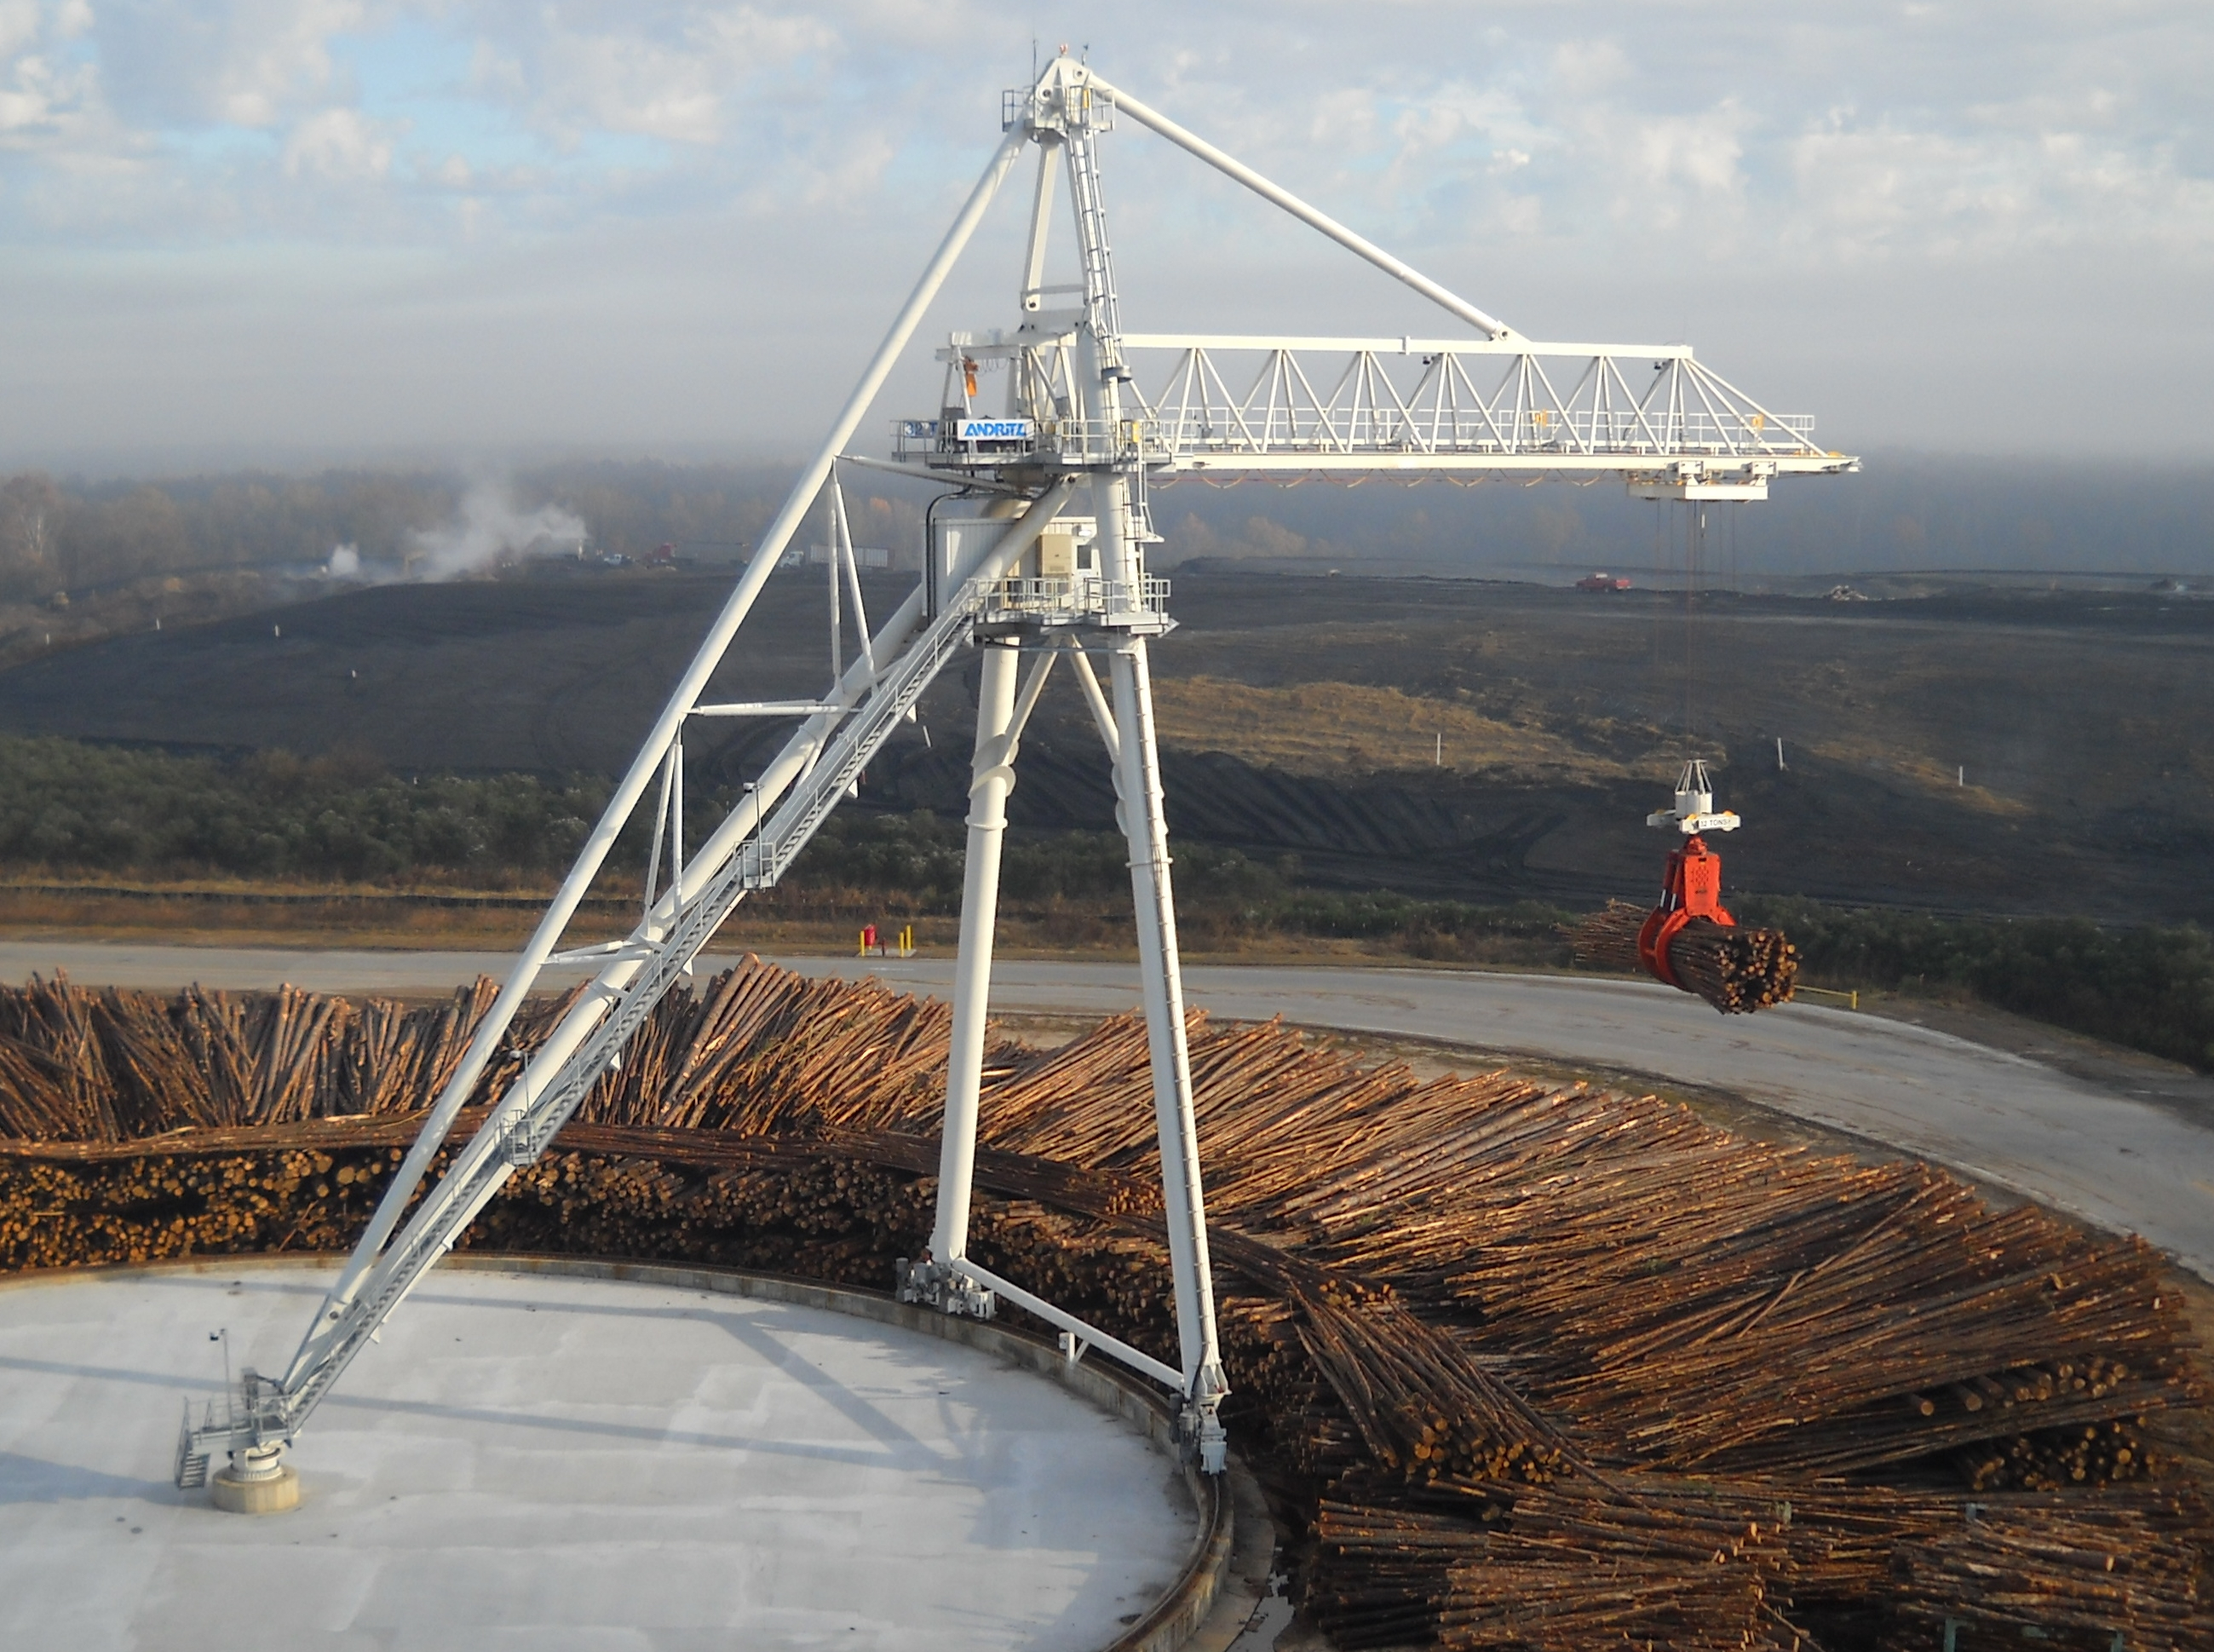
\includegraphics[width=0.5\textwidth, center]{bilder/Grundlagen/Kran_vollstaendig_N1_030.jpg}
		\caption[Rund-Kran]{Rundlaufkran (Foto: ANDRITZ)}
		\label{img:CircularCrane}
	\end{figure}		

	\paragraph{Greifer-Erkennung} 
	Zur Lösung der Aufgaben wird unter anderem ein neuronales Netzwerk zur Positionserkennung des Greifers eingesetzt. Für diese Arbeit werden Vorhersagen des Netzes als Vergleichswert für die Versuche genutzt. Das Netz liegt als frozen\_inference\_graph.pb vor. Zur Erzeugung des Neuronalen Netzwerkes wurde auf die Technik des Single Shot MultiBox Detector [todo https://arxiv.org/abs/1512.02325] zurückgegriffen. Protocoll Buffer  [https://developers.google.com/protocol-buffers/] ist ein sprachneutraler, plattformneutraler, erweiterbarer Mechanismus zur Serialisierung strukturierter Daten. In diesem Fall enthält die Datei den eingefrorenen Graph und die Model Gewichte. Vorhersagen können mittels einer Tensorflowsession getroffen werden. Dabei liefert das Model, Rahmen in welchem sich der Greifer befindet und einen Vertrauenswert der aussagt wie sicher sich das Netzt mit seiner Aussage ist.	[https://leimao.github.io/blog/Save-Load-Inference-From-TF-Frozen-Graph/]
		
	\paragraph{Baumstamm-Klassifikation} 
	Ein Klassifikatior, für die Frage ob sich Baumstämme in dem Greifer befinden liegt als meta\_graph vor. Die Vorhersage des Modells liefert die vorhergesagte Klasse mit einer Wahrscheinlichkeit zurück.

	\section{Datenverständnis}
	\label{sec:DataUnderstanding}
	Anlehnend dem in Kapitel \ref{sec:Vorgehen} beschriebenen Vorgehen \todo{Vorgehen auch so beschreiben /  ansonsten Kapitel Einleitung anpassen} werden in diesem Kapitel die zur Verfügung stehenden Daten und deren Qualität beschrieben. Dabei ist das Kapitel entsprechend der Beschriftung der Daten in zwei Teilbereiche unterteilt.
	
	Im Rahmen des Autocrane-Projektes \ref{sec:BestehendesSystem} \todo{Im Kapitel Bestehdens System erwähnen / diesen Teil in das andere Kapitel verschieben?} wurde eine Kamera an einem Rundlaufkran angebracht. Die Kamera ist so ausgerichtet, dass sich Aufhängung des Greifers am mittleren oberen Bildrand befindet. Bei einem Rundlaufkran kann die Auslenkung komplett um das Zentrum des Krans bewegt werden. Der Hintergrund der Bilder kann sich stark ändern. Mittels der Kamera werden kontinuirlich neue unbeschriftete Bilder aufgenommen und bei PSIORI abgelegt. Zu Beginn dieser Arbeit standen mehr 385.000 nicht beschriftete Bilder zur Verfügung. Die Bilder sind 1024 auf 648 Pixel groß und in Farbe. Sie sind in der Form (1024, 648, 3). Die einzelnen Pixel können dabei Werte zwischen 0 und 255 annehmen. 
	Zum Erreichen der Zielstellung werden zwei Datensätze benötigt.
	
		\paragraph{Greifer Datensatz} Der Greifer Datensatz enthält Bilder, in welchen der Greifer mittels Rahmen markiert ist. Abbildung \ref{img:Logs}  zeigt ein beispielhaftes Bild mit markiertem Greifer. Abbildung \ref{img:Grapple} zeigt ein beispielhaftes Bild mit markiertem Greifer.
		\begin{figure}[h]
				\centering
				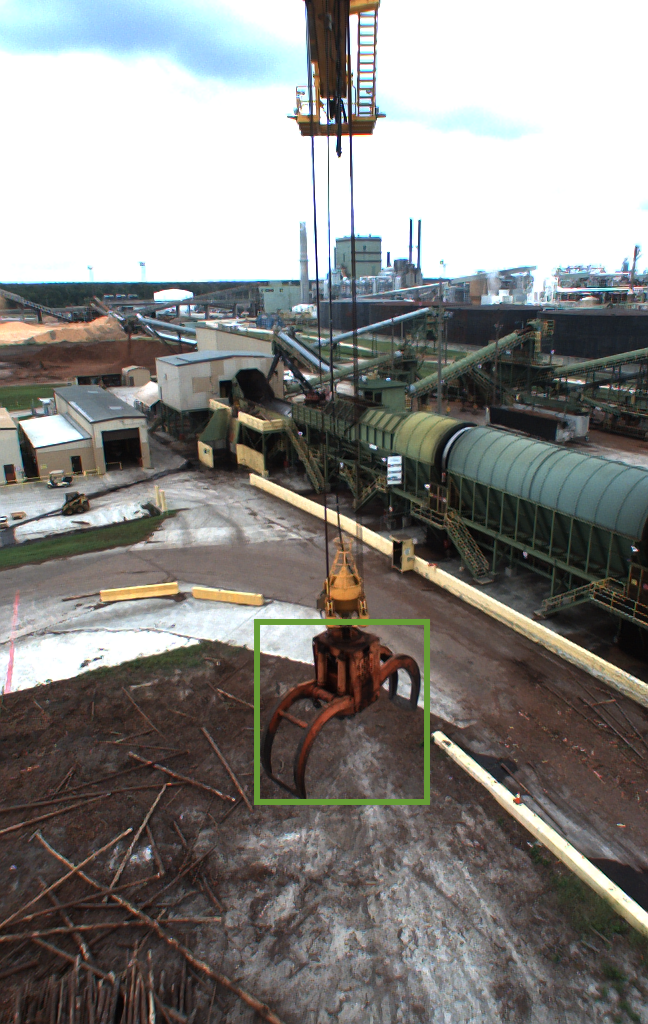
\includegraphics[width=0.5\textwidth, center]{bilder/Grundlagen/Grapple_8.png}
				\caption[Bsp. Bild: Greifer mit Rahmen]{Greifer mit Rahmen}
				\label{img:Grapple}
		\end{figure}
		Der Datensatz besteht aus zwei Sammlungen von qualitativ unterschiedlich gut beschrifteten Bildern. Die eine Sammlung besteht aus einem bestehenden Datensatz, welcher 4.684 durch Menschen annotierten Bildern enthält. Für den zweiten Teil der Sammlung wurden mittels der bestehenden Objekterkennung 14.018 Bilder annotiert. 
		
		\paragraph{Baumstamm Datensatz} Der Baumstamm Datensatz enthält Bilder, welche die Annotation, ob sich Baumstämme im Greifer befinden haben. Abbildung \ref{img:Logs} zeigt ein Bild, in welchem der Greifer Baumstämme greift. In Abbildung \ref{img:Grapple} befinden sich keine Baumstämme im Greifer.
		\begin{figure}[h]
			\centering
			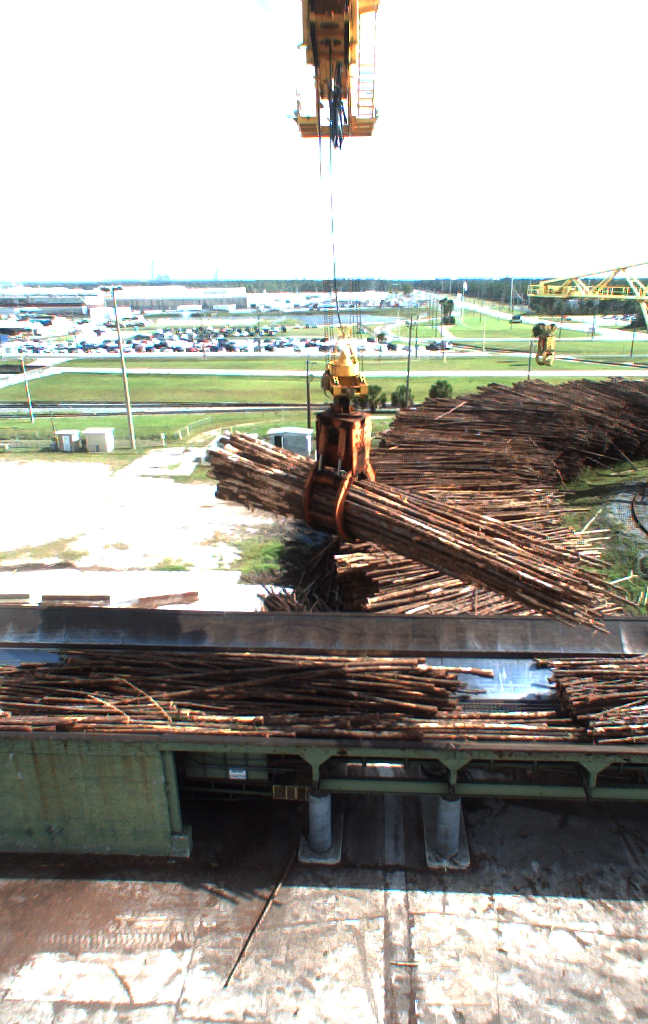
\includegraphics[width=0.5\textwidth, center]{bilder/Grundlagen/Logs_14.png}
			\caption[Bsp. Bild: Greifer mit Baumstämmen]{Greifer mit Baumstämmen}
			\label{img:Logs}
		\end{figure}
		Der Datensatz wurde im Zusammenarbeit mit quality-match[https://www.quality-match.com/imprint] und Crowdworkern erstellt.  

		\paragraph{Weiterer Datensatz}
		Im laufe der Arbeit wurden in Zusammenarbeit mit quality-match ein weiterer Datensatz erstellt. Dieser Datensatz enthält \todo{finale Zahl setzen} 80.000 beschriftete Bilder. Es wurden sowohl die Beschriftung "Logs ja / nein" als auch die Beschriftung  Rahmen des Greifers erstellt. Zusätzlich wurden weitere Beschriftungen wie Hellichkeit, Winkel des Greifers, ... erstellt. Dieses weiteren Beschriftungen wurden in der Arbeit nicht genutzt.		\todo{stimmt das am Ende noch?}
	
		
	\section{Datenvorbereitung}
	\label{sec:DataPreparation}

Die Datenvorbereitung dient dazu, einen finalen Datensatz zu erstellen, der die Basis für die nächste Phase der Modellierung bildet.


			In dem Schritt Datenvorbereitung werden die Bilder für die Modellerstelung vorbereitet. In dieser Arbeit wurde für diesen Schritt eine Klasse Preprocessing in einem neuen Modul data\_preperation.py  erstellt. Wie in Listing 
			% \lstinputlisting[language=Python,caption={Preprocessing},label=lst:Preprocessing]{\srcloc/data\_preperation.py }
			
			 zu sehen werden die Pixel der Bilder zwischen 0 und 1 Skaliert. Dei Skalierung erfolgt damit jedes Bild eine ähnliche Gewichtung
			
			Neural networks process inputs using small weight values, and inputs with large integer values can disrupt or slow down the learning process. As such it is good practice to normalize the pixel values so that each pixel value has a value between 0 and 1.
			
			Die Bilddaten werden 		
			

 

	\begin{table}[ht]
	\centering
	\begin{tabularx}{\textwidth}{lllll}
		 & \textbf{Train} & \textbf{Test}  & \textbf{Validation} & \textbf{Summe} 	 \\
		\textbf{Greifer} 				 & 	3.279			& 703	 & 704				   & 4.686 	\\
		\textbf{Baumstämme j/n}	 	  &  9.749	   & 1.221 	& 1.225	& 12.195\\
		
	\end{tabularx}
	\caption{Datenaufteilung - Train Test Validation}
	\label{table:DatenaufteilungTrainTestValidation}
 	\end{table}
 
